\begin{table*}[ht]
	\footnotesize
	\begin{center}
		{
			\setlength\tabcolsep{4.5pt}
			\renewcommand{\arraystretch}{1.5}
			\begin{tabular}{c|c|c|c|c|c|c|c|c|c|c|c|c|c|c|c|c}
				\hline
				& orig& gauss& shot& impul& defoc& glass& motn& zoom& snow& frost& fog& brit& contr& elast& pixel& jpeg\\
				\hline
				TTT-Online & \textbf{8.2}& \textbf{25.8}& \textbf{22.6}& 30.6& \textbf{14.6}& \textbf{34.4}& \textbf{18.3}& \textbf{17.1}& \textbf{20.0}& \textbf{18.0}& \textbf{16.9}& \textbf{11.2}& 15.6& \textbf{21.6}& \textbf{18.1}& \textbf{21.2}\\
				\hline
				UDA-SS & 9.0& 28.2& 26.5& \textbf{20.8}& 15.6& 43.7& 24.5& 23.8& 25.0& 24.9& 17.2& 12.7& \textbf{11.6}& 22.1& 20.3& 22.6\\
				\hline
			\end{tabular}
			\renewcommand{\arraystretch}{1}
		}
	\end{center}
	\caption{
		{\bf Test error (\%) on CIFAR-10-C with level 5 corruption.} Comparison between online Test-Time Training (TTT-Online) and unsupervised domain adaptation by self-supervision (UDA-SS)~\citep{sun2019uda} with access to the entire (unlabeled) test set during training. We highlight the lower error in bold. We have abbreviated the names of the corruptions, in order: original test set, Gaussian noise, shot noise, impulse noise, defocus blur, glass blue, motion blur, zoom blur, snow, frost, fog, brightness, contrast, elastic transformation, pixelation, and JPEG compression. 
		The reported numbers for TTT-Online are the same as in \autoref{fig:cc}.
		See complete table in \autoref{table:full_c10c}.
	}
\label{table:uda}
\end{table*} 
\begin{figure*}[ht]
	\centering
	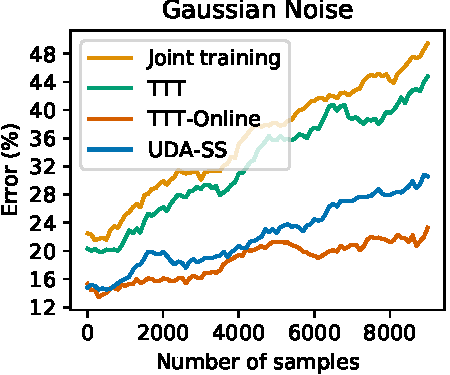
\includegraphics[width=0.33\textwidth]{plots/smooth/gaussian_noise_12345_avg.pdf}
	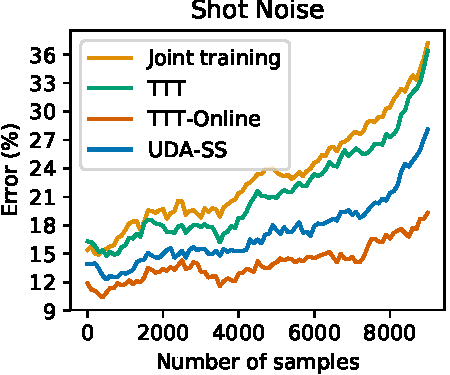
\includegraphics[width=0.33\textwidth]{plots/smooth/shot_noise_12345_avg.pdf}
	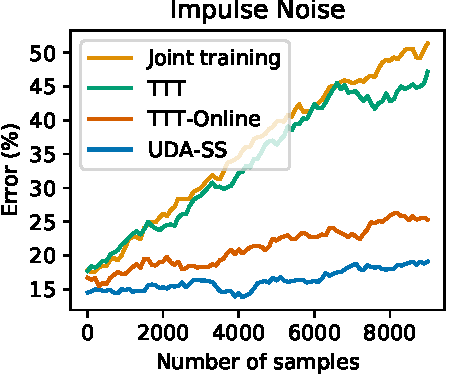
\includegraphics[width=0.33\textwidth]{plots/smooth/impulse_noise_12345_avg.pdf}
    
	\caption{
		{\bf Test error (\%) on CIFAR-10-C, for the three noise types, with gradually changing distribution.}
		The distribution shifts are created by increasing the standard deviation of each noise type from small to large, the further we go on the x-axis. As the samples get noisier, all methods suffer greater errors the more we evaluate into the test set, but online Test-Time Training (TTT-Online) achieves gentler slopes than joint training. For the first two noise types, TTT-Online also achieves better results over unsupervised domain adaptation by self-supervision (UDA-SS)~\citep{sun2019uda}.
	}
	\label{fig:smooth}
% 	\vspace{-2ex}
\end{figure*}